\documentclass[10pt,letterpaper]{amspset}
\usepackage{fullpage}
\usepackage{gensymb}
\usepackage{graphicx}
\usepackage{tikz}
\graphicspath{ {./images/} }
\notag

%notice the use of the \newcommand command.  It's making your life a little easier by defining commands that you can use later.
\newcommand{\R}{\mathbb{R}}
\newcommand{\Q}{\mathbb{Q}}
\newcommand{\Z}{\mathbb{Z}}
\newcommand{\N}{\mathbb{N}}

% info for header block in upper right hand corner
\name{Brady Lamson}
\class{MATH 1120 SPRING 2021}
\assignment{Homework Part 2}
\duedate{Jan 31st}



\begin{document}

\problemlist{Radian and Degree Measures Part 2: Problems 45-49, 52-56, 59-63 }

In exercises 45-49, sketch the oriented arc on the Unit Circle which corresponds to the given real number.

\begin{problem} [45.]
$t = \frac{5\pi}{6}$
\end{problem}

\begin{solution}
This one is very similar to the earlier problems in Part 1. $t= \frac{5\pi}{6}$ is very close to $1\pi$. This lands it nicely in Quadrant 2. To make certain I was right I did a few quick calculations to prove it.

\begin{align}
    \pi &= 3.14 \\
    \frac{1\pi}{2} &= 1.57 \\
    \frac{5\pi}{6} &= 2.617 \\
    1.57 < 2.617 &< 3.14
\end{align} 

\begin{center}
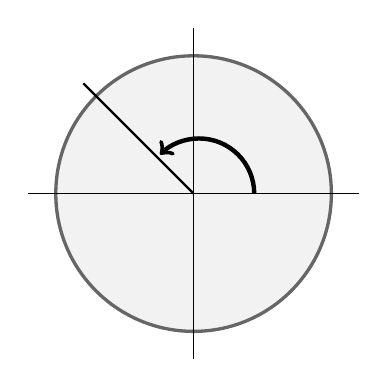
\begin{tikzpicture}[scale=0.7]
        \filldraw[color=black!60, fill=black!5, very thick](0,0) circle (2.5);
        \draw (-3,0) -- (3,0);
        \draw (0,3) -- (0,-3);
        \draw [thick ] (0,0) -- (-2,2);
        \draw[ultra thick, ->] (1.1,0) arc (0:135:1);
    \end{tikzpicture}
\end{center}
\end{solution}


\begin{problem} [46.]
$t = -\pi$
\end{problem}

\begin{solution}
This one is incredibly straightforward. All you need to do is go to $\pi$ in a clockwise direction which is in the same location as $180\degree$.
\begin{align}
    x &= -\pi \left(\frac{180\degree}{\pi}\right) \\
    x &= -180\degree
\end{align}

\begin{center}
    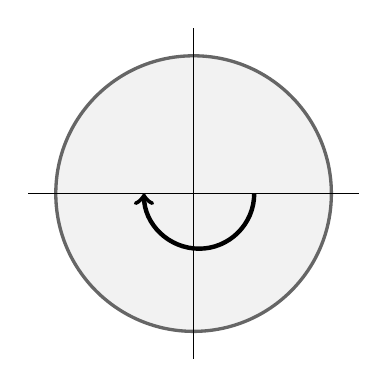
\begin{tikzpicture}[scale=0.7]
        \filldraw[color=black!60, fill=black!5, very thick](0,0) circle (2.5);
        \draw (-3,0) -- (3,0);
        \draw (0,3) -- (0,-3);
        \draw[ultra thick, ->] (1.1,0) arc (0:-180:1);
    \end{tikzpicture}
\end{center}
\end{solution}



\begin{problem} [47.]
$t = 6$
\end{problem}

\begin{solution}
On the surface this seems very different than the other values. There isn't a $\pi$ value to gauge where it ends up on the circle. That is until you realize that the radian measure is just another way to represent a real number. Once you realize that $\pi = 3.14$ it becomes quite clear how to map numbers like $6$ onto the circle. Since $2\pi = 6.28$ it stands to reason that $t=6$ would likely end up in quadrant 3. Let's do some comparisons.

\begin{align}
    \frac{3\pi}{2} &= 4.71 \\
    2\pi &= 6.28 \\
    4.71 < 6 &< 6.28
\end{align} 

\begin{center}
    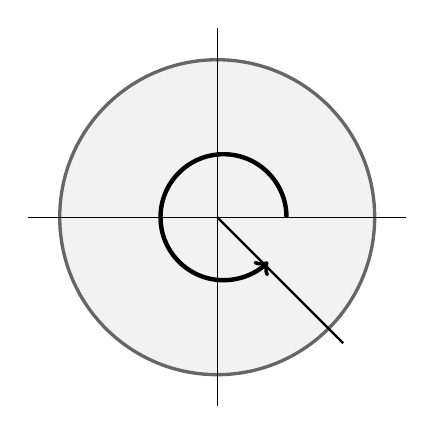
\begin{tikzpicture}[scale=0.8]
        \filldraw[color=black!60, fill=black!5, very thick](0,0) circle (2.5);
        \draw (-3,0) -- (3,0);
        \draw (0,3) -- (0,-3);
        \draw [thick ] (0,0) -- (2,-2);
        \draw[ultra thick, ->] (1.1,0) arc (0:315:1);
    \end{tikzpicture}
\end{center}
\end{solution}

\begin{problem} [48.]
$t = -2$
\end{problem}

\begin{solution}
We can use the same logic as we did in the previous problem. The only difference is that we have to take the negative into account. After doing the comparisons it becomes clear that $t = -2$ falls into quadrant 3. 

\begin{align}
    -\pi &= -3.14 \\
    -\frac{1\pi}{2} &= -1.57 \\
    -1.57 > -2 &> -3.14
\end{align} 

\begin{center}
    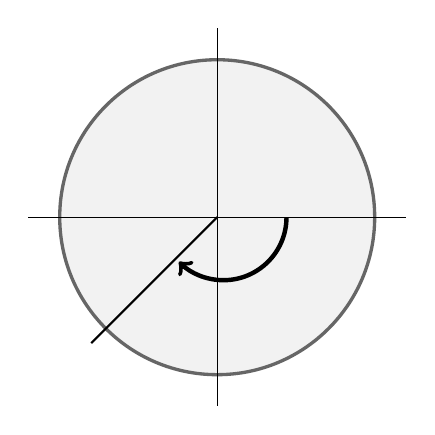
\begin{tikzpicture}[scale=0.8]
        \filldraw[color=black!60, fill=black!5, very thick](0,0) circle (2.5);
        \draw (-3,0) -- (3,0);
        \draw (0,3) -- (0,-3);
        \draw [thick ] (0,0) -- (-2,-2);
        \draw[ultra thick, ->] (1.1,0) arc (0:-135:1);
    \end{tikzpicture}
\end{center}

\end{solution}


\begin{problem} [49.]
$t = 12$
\end{problem}

\begin{solution}
Now we have to start doing comparisons to values higher than one rotation. This is fairly straightforward and we find that $t=12$ comes very close to completing two full rotations. This lands it in quadrant 4.

\begin{align}
    4\pi &= 12.56 \\
    \frac{7\pi}{2} &= 10.99 \\
    10.99 < 12 &< 12.56
\end{align} 

\begin{center}
    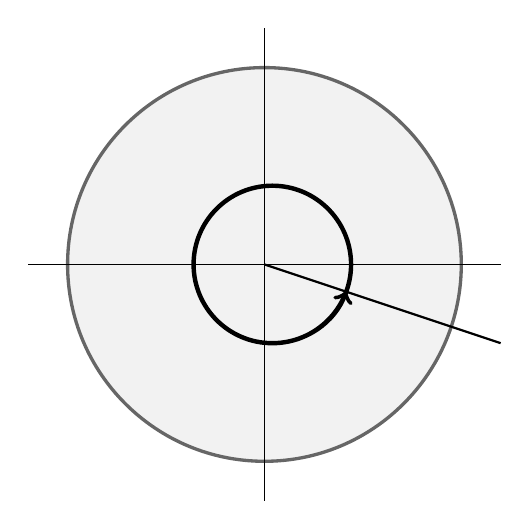
\begin{tikzpicture}
        \filldraw[color=black!60, fill=black!5, very thick](0,0) circle (2.5);
        \draw (-3,0) -- (3,0);
        \draw (0,3) -- (0,-3);
        \draw [thick ] (0,0) -- (3,-1);
        \draw[ultra thick, ->] (1.1,0) arc (0:700:1);
    \end{tikzpicture}
\end{center}

\end{solution}


\pagebreak


\begin{problem}[52.]
In  the  yo-yo  trick  ‘Around  the  World,’  the  performer  throws  the  yo-yo  so  it  sweeps  out  a vertical circle whose radius is the yo-yo string.  If the yo-yo string is 28 inches long and the yo-yo takes 3 seconds to complete one revolution of the circle, compute the speed of the yo-yo in miles per hour.  Round your answer to two decimal places
\end{problem}

\begin{solution}
Before we start we must state our given information.
\[r = 28in\]
\[t = 3 seconds\]
Both of these values need to be converted, $r$ to miles and $t$ to hours. Let's start with $r$. There are $63360$ inches per mile.

\begin{align}
    r &= 28in \left(\frac{1m}{63360in}\right) \\
    r &= 4.4 * 10^{-4}miles
\end{align}

\noindent Next we convert $t$ to hours. There are 60 seconds per minute and 60 minutes per hour. 

\begin{align}
    t &= 3s * \left(\frac{1m}{60s}\right) * \left(\frac{1h}{60m}\right) \\
    t &= 8.3 * 10^-4 hours
\end{align}

\noindent Since we're trying to calculate the speed of the yo-yo we can use the formula below. This formula is used assuming constant angular velocity $\omega$. 

\[v = r * \omega\]

Velocity (v) is in units of $\frac{miles}{hour}$, radius (r) is in miles and $\omega$ is in units of $\frac{radians}{hour}$. From here we really can just plug and chug. 

\begin{align}
    v &= r * \omega \\
    r &= 4.4 * 10^{-4}m \\
    t &= 8.3 * 10^{-4}h \\
    \omega &= \frac{2\pi}{8.3 * 10^{-4}h} \\[+3mm]
    \omega &= \frac{\pi}{4.15 * 10^{-4}h} \\[+3mm]
    v &= \frac{4.4 *10^-4m * \pi}{4.15 * 10^{-4}h} \\[+3mm]
\end{align}

\[\boxed{v &= 3.33\frac{miles}{hour}}\]

\end{solution}


\pagebreak


\begin{problem} [53.]
A computer hard drive contains a circular disk with diameter 2.5 inches and spins at a rate
of 7200 RPM (revolutions per minute). Find the linear speed of a point on the edge of the
disk in miles per hour.
\end{problem}

\begin{solution}
\begin{align}
    d &= 2.5in \\
    \omega &= \frac{7200 * 2\pi}{1minute}
\end{align}

We first have to do all of our conversions. Our diameter needs to be divided by 2 to get the radius and then needs to be converted to miles. We also need to convert the minutes in $\omega$ to hours. 

\begin{align}
    d &= 2.5in \\[+3mm]
    r &= \frac{1}{2}d \\[+3mm]
    r &= 1.25in \\[+3mm]
    r &= 1.25in \left(\frac{1m}{63360in}\right) \\[+3mm]
    r &= 1.97 * 10^{-5}miles \\[+3mm]
    t &= 1 min * \frac{1hour}{60min} \\[+3mm]
    t &= 0.0167hours
\end{align}

From here we plug and chug.

\begin{align}
    r &= 1.97 * 10^{-5}miles \\[+3mm]
    t &= 0.0167hours \\[+3mm] 
    \omega &= \frac{7200 * 2\pi}{0.0167hours} \\[+3mm]
    v &= r * \omega \\[+3mm]
    v &= (1.97 * 10^{-5}miles) * \left(\frac{7200 * 2\pi}{0.0167hours} \right) \\[+3mm]
\end{align}

\[\boxed{v = 53.47 \frac{miles}{hour}}\]
\end{solution}

\pagebreak


\begin{problem}[54.]
A rock got stuck in the tread of my tire and when I was driving 70 miles per hour, the rock
came loose and hit the inside of the wheel well of the car. How fast, in miles per hour, was
the rock traveling when it came out of the tread? (The tire has a diameter of 23 inches.)
\end{problem}

\begin{solution}[Solution]
I believe that this is a trick question. The velocity of the car is given and based on the information given there is no reason to assume that the velocity of the rock would be any different. If it is different then that would likely start to get into physics and we would need far more values given to work through that. 

\[\boxed{v = 70\frac{miles}{hour}}\]
\end{solution}


\begin{problem}[55.]
The Giant Wheel at Cedar Point is a circle with diameter 128 feet which sits on an 8 foot tall
platform making its overall height is 136 feet. It completes two revolutions in 2 minutes and 7 seconds. Assuming the riders are at the edge of the circle, how fast are they traveling in miles per hour?
\end{problem}

\begin{solution}[Solution]
I'm fairly confident thinking that we can ignore the platform and height of the wheel. We will quickly find out. Let us solve this the same as every other problem. 

\begin{align}
    d &= 128ft \\
    r &= 64ft \\
    t &= 2m7s \\
    \omega &= \frac{2 * (2\pi)}{t} \\
\end{align}

You know the drill, it's time for some conversions. We need $r$ in miles and $t$ in hours.

\begin{align}
    r &= 64ft \left( \frac{1mile}{5280ft} \right) \\[+1mm]
    r &= 0.012miles \\[+2mm]
    t &= 2minutes7seconds \\[+2mm]
    7sec &= \frac{7}{60} = 0.1167 \\[+2mm]
    t &= 2.1167min * \left( \frac{1hour}{60min} \right) \\[+2mm]
    t &= 0.035hours \\[+2mm]
    v &= r * \omega \\
    v &= 0.012miles * \left( \frac{2 * (2\pi}{0.035} \right) \\
    \end{align}
    
\[\boxed{v = 4.31 \frac{miles}{hour}}\]
\end{solution}


\begin{problem}[56.]
Consider the circle of radius r pictured below with central angle $\theta$, measured in radians, and subtended arc of length s. Prove that the area of the shaded sector is $A = \frac{1}{2} r^2 \theta$.  
Hint: Use the proportion $\frac{A}{A_c} = \frac{s}{circumference}$
\end{problem}

\begin{solution}[Solution]
Before we can start let me provide the units I will be using.  

\begin{align}
    A &= Area \\
    A_c &= \textrm{Area of circle} \\
    s &= \textrm{subtend arc} \\
    r &= radius \\
    d &= diameter \\
    c &= circumference \\
    A_c &= \pi r^2 \\
    \frac{A}{A_c} &= \frac{s}{c} \\
    c &= \pi * d \\
    d &= 2 * r \\
    s &= \theta * r \\ 
\end{align}

Here I'm going to substitute some values to list off some equivalencies.
\begin{align}
    \frac{A}{\pi * r^2} &= \frac{s}{\pi * d} \\[+3mm]
    \frac{s}{\pi * d} &= \frac{s}{2 \pi  r} \\[+3mm]
    \frac{A}{\pi r^2} &= \frac{s}{2 \pi  r} \\[+3mm]
    \frac{A}{\pi r^2} &= \frac{s}{2 \pi  r} \\[+3mm]
    A &=\frac{s \pi r^2}{2 \pi r} \\[+3mm]
    A &= \frac{1}{2} r s
\end{align}

Keep in mind that $s = \theta r$. With that taken into account let's substitute that into our final equation!
\[\boxed{A = \frac{1}{2} r^2 \theta}\]
\end{solution}

\pagebreak


\begin{problem}[57.]
$\theta = \frac{\pi}{6}, r = 12$
\end{problem}

\begin{solution}[Solution]
Since we did the hard part already for the next few problems all we need to do is plug and chug.

\begin{align}
    A &= \frac{1}{2} r^2 * \theta \\[+3mm]
    A &= \frac{1}{2} 12^2 * \frac{\pi}{6} \\[+3mm]
    A &= \frac{1 * 12^2 * \pi}{2 * 6} \\[+3mm]
    A &= \frac{12^2 * \pi}{12} \\[+3mm]
\end{align}
\[\boxed{A = 12 \pi = 37.699}\]
\end{solution}


\begin{problem}[59.]
$\theta = 330\degree, r = 9.3$
\end{problem}

\begin{solution}[Solution]
Not much more to say here, we just need to convert from degrees to radians.

\begin{align}
    \theta &=\frac{330\degree}{1} * \frac{\pi}{180\degree} \\[+3mm]
    A &= \frac{1}{2} r^2  \theta \\[+3mm]
    A &= \frac{1}{2} 9.3^2 * \frac{330\degree * \pi}{180\degree} \\[+3mm]
    A &= \frac{1 * 9.3^2 * 330\degree \pi}{180\degree * 2} \\[+3mm]
\end{align}
\[\boxed{A = 79.28 \pi = 249.07}\]
\end{solution}

\pagebreak


\begin{problem}[60.]
$\theta = \pi, r = 1$
\end{problem}

\begin{solution}[Solution]

\begin{align}
    A &= \frac{1}{2} r^2  \theta \\[+3mm]
    A &= \frac{1}{2} 1^2 * \pi \\[+3mm]
    A &= \frac{1 * 1^2 * \pi}{2} \\[+3mm]
\end{align}
\[\boxed{A = \frac{1}{2}\pi = \frac{\pi}{2}}\]
\end{solution}


\begin{problem}[61.]
$\theta = 240\degree, r = 5$
\end{problem}

\begin{solution}[Solution]

\begin{align}
    \theta &=\frac{240\degree}{1} * \frac{\pi}{180\degree} \\[+3mm]
    A &= \frac{1}{2} r^2  \theta \\[+3mm]
    A &= \frac{1}{2} 5^2 * \frac{240\degree * \pi}{180\degree} \\[+3mm]
    A &= \frac{1 * 5^2 * 240\degree \pi}{180\degree * 2} \\[+3mm]
\end{align}
\[\boxed{A = 16.67 \pi = 52.36}\]
\end{solution}


\begin{problem}[62.]
$\theta = 1\degree, r = 117$
\end{problem}

\begin{solution}[Solution]

\begin{align}
    A &= \frac{1}{2} r^2  \theta \\[+2mm]
    A &= \frac{1}{2} 117^2 * \frac{1\degree * \pi}{180\degree} \\[+2mm]
    A &= \frac{1 * 117^2 * 1\degree \pi}{180\degree * 2} \\[+2mm]
\end{align}
\[\boxed{A = 38.025 \pi = 119.46}\]
\end{solution}


\begin{problem}[63.]
Imagine a rope tied around the Earth at the equator. Show that you need to add only $2\pi$ feet of length to the rope in order to lift it one foot above the ground around the entire equator.
(You do NOT need to know the radius of the Earth to show this.)
\end{problem}

\begin{solution}[Solution]
First we must state our givens. For this we can visualize two circles, one representing the earth and the other representing the rope going around the equator. We will have $C_0$ represent the circumference of the earth and $C_1$ will represent the circumference of the rope. We will also have $r_0$ and $r_1$ representing the radius of the two circles.  

So, using those givens we can state that the circumference of the earth can be calculated using the formula $C_0 = 2 \pi r_0$. Now, $C_1$ is a little different. Its radius is $r_1$ and $C_1$ is $2\pi$ longer than $C_0$. This can be represented as follows:

\[C_1 = C_0 + 2\pi = 2 \pi r_1\]

Now we substitute $C_0$ for what makes it up. This gives us the following formula.

\[C_1 = 2\pi r_0 + 2\pi = 2\pi r_1\]

Now we can take out the $2 \pi$.

\[C_1 = 2 \pi ( r_0 + 1 ) = 2 \pi (r_1)\]

Therefore:

\[\boxed{r_0 + 1 = r_1} \]

\end{solution}

\end{document}